% ============================================================
%  Module 7 — The Solow Growth Model
%  From Smith to Simulation · University of Edinburgh
% ============================================================
\documentclass[aspectratio=169, 10pt]{beamer}
\usetheme{metropolis}

% --- Edinburgh colours ----------------------------------------
\definecolor{UoERed}{HTML}{7A2318}
\definecolor{UoEGold}{HTML}{B8860B}
\definecolor{CodeBG}{HTML}{F7F3ED}
\definecolor{CodeFrame}{HTML}{D5C9B1}

\setbeamercolor{palette primary}{bg=UoERed, fg=white}
\setbeamercolor{frametitle}{bg=UoERed, fg=white}
\setbeamercolor{title separator}{fg=UoEGold}
\setbeamercolor{progress bar}{fg=UoEGold, bg=UoEGold!20}
\setbeamercolor{alerted text}{fg=UoERed}
\setbeamercolor{block title}{bg=UoERed!15, fg=UoERed}
\setbeamercolor{block body}{bg=UoERed!5}

% --- Packages -------------------------------------------------
\usepackage[T1]{fontenc}
\usepackage{lmodern}
\usepackage{amsmath, amssymb, mathtools}
\usepackage{listings}
\usepackage{graphicx, booktabs}
\usepackage{tikz}
\usetikzlibrary{arrows.meta, positioning, calc, decorations.pathreplacing}
\usepackage{hyperref}
\hypersetup{colorlinks=true, linkcolor=UoERed, urlcolor=UoERed!70!black}
\setbeamertemplate{navigation symbols}{}

\lstset{
  language=Python,
  basicstyle=\ttfamily\scriptsize,
  keywordstyle=\color{UoERed}\bfseries,
  commentstyle=\color{gray}\itshape,
  stringstyle=\color{UoEGold},
  backgroundcolor=\color{CodeBG},
  frame=single,
  rulecolor=\color{CodeFrame},
  numbers=none,
  breaklines=true,
  showstringspaces=false,
  tabsize=4,
  xleftmargin=4pt, xrightmargin=4pt,
  aboveskip=6pt, belowskip=4pt,
}

% Section title pages
\AtBeginSection[]{
  \begin{frame}
    \vfill\centering
    \usebeamerfont{title}\insertsectionhead\par
    \vfill
  \end{frame}
}

% ---- Title ---------------------------------------------------
\title{Module 7 --- The Solow Growth Model}
\subtitle{Capital Accumulation, Steady States, and the Sources of Growth}
\author{Dr Juan Zurita}
\institute{From Smith to Simulation\\
The University of Edinburgh~$\cdot$~School of Economics}
\date{}

\begin{document}

% =============================================================
\maketitle
% =============================================================

% -------------------------------------------------------------
\section{Part I --- The History}
% -------------------------------------------------------------

\begin{frame}{Post-War Prosperity and an Unanswered Question}
\begin{columns}[T]
\column{0.55\textwidth}
After 1945 the world economy experienced unprecedented growth:
\begin{itemize}
  \item Western Europe rebuilt from rubble in a single generation.
  \item The US doubled living standards between 1945 and 1970.
  \item Japan rose from wartime devastation to the world's second-largest economy.
  \item West Germany's \textit{Wirtschaftswunder} tripled real GDP per capita
        (1950--1970).
\end{itemize}
\column{0.4\textwidth}
\begin{block}{The Open Question}
Where did all this growth come from?
Smith, Ricardo, and Marx had theories of value but
\textbf{no formal model of how economies grow over time}.
Keynes explained fluctuations but said little about the
\alert{long-run trajectory}.
\end{block}
\end{columns}
\end{frame}

\begin{frame}{The Harrod--Domar Problem}
In the late 1940s, Roy Harrod and Evsey Domar independently proposed
growth models:
\vspace{0.5em}
\begin{itemize}
  \item Growth depends on the \textbf{saving rate} and the
        \textbf{capital--output ratio}.
  \item But the models had a fatal flaw: the growth path was
        \alert{knife-edge unstable}.
  \item Any deviation from the ``warranted rate'' led to ever-widening
        booms or slumps.
  \item No diminishing returns $\Rightarrow$ no self-correcting mechanism.
\end{itemize}
\vspace{0.5em}
The economics profession needed a model where growth was
\textbf{stable} --- where the economy would naturally settle
at a sustainable path.
\end{frame}

\begin{frame}{Robert Solow and the 1956 Paper}
\begin{columns}[T]
\column{0.55\textwidth}
In 1956, \textbf{Robert Solow} (1924--2023) at MIT published
\textit{``A Contribution to the Theory of Economic Growth''}.
\vspace{0.5em}
\begin{enumerate}
  \item Output is produced from \textbf{capital} and \textbf{labour}
        via a production function.
  \item A fixed fraction of output is \textbf{saved and invested}.
  \item Capital \textbf{depreciates} --- machines wear out.
  \item The production function exhibits \alert{diminishing returns}
        to capital.
\end{enumerate}
\column{0.4\textwidth}
\begin{block}{The Startling Conclusion}
Capital accumulation \textbf{alone} cannot sustain long-run growth.
Because of diminishing returns, each new unit of capital adds less
output. The economy settles at a \alert{steady state}.
\end{block}
\end{columns}
\end{frame}

\begin{frame}{Solow's Key Insight}
\begin{center}
\textit{``All theory depends on assumptions which are not quite true.
That is what makes it theory. The art of successful theorizing is to
make the inevitable simplifying assumptions in such a way that the
final results are not very sensitive.''}\\[6pt]
--- Robert Solow, \textit{Quarterly Journal of Economics} (1956)
\end{center}
\vspace{1em}
\begin{itemize}
  \item By adding \textbf{diminishing returns}, Solow turned Harrod--Domar's
        knife-edge into a \alert{globally stable} steady state.
  \item The model is simple enough to solve analytically, yet rich enough
        to explain the major facts of post-war growth.
\end{itemize}
\end{frame}

\begin{frame}{The Solow Residual: Technology as the True Engine}
Solow's empirical companion paper (1957) decomposed US growth
(1909--1949):
\vspace{0.5em}
\begin{columns}[T]
\column{0.48\textwidth}
\begin{block}{The Decomposition}
  \begin{itemize}
    \item Capital and labour together explained only
          $\approx$\textbf{12.5\%} of output growth.
    \item The remaining \alert{87.5\%} was a \textbf{residual}.
  \end{itemize}
\end{block}
\column{0.48\textwidth}
\begin{block}{Total Factor Productivity}
  The residual captures:
  \begin{itemize}
    \item Technological progress
    \item Better management
    \item Improved institutions
    \item Education and innovation
  \end{itemize}
\end{block}
\end{columns}
\vspace{0.5em}
Solow's message: \textit{technology, not saving,
is the true engine of long-run growth.}
\end{frame}

\begin{frame}{The Growth Miracles}
Solow's framework explains the post-war miracles:
\vspace{0.5em}
\begin{description}
  \item[\textbf{Germany \& Japan}] Started with capital stocks destroyed
        but human capital intact.
        Low $k \Rightarrow$ enormous returns to investment $\Rightarrow$
        rapid convergence toward steady state.
  \item[\textbf{Asian Tigers}] South Korea, Taiwan, Hong Kong, Singapore
        followed a similar path from the 1960s onward.
\end{description}
\vspace{0.5em}
The model also predicted that rapid growth would \alert{slow} as
countries approached their steady states --- which is precisely
what happened.
\end{frame}

\begin{frame}{Edinburgh Connection and the Nobel Prize}
\begin{itemize}
  \item The Scottish Enlightenment's commitment to \textbf{empirical inquiry}
        --- from Hume's insistence on observation to Smith's systematic
        evidence --- laid the groundwork for quantitative growth economics.
  \item Solow's method of \textbf{confronting theory with data},
        decomposing growth into measurable components, and letting
        the residual speak for itself embodies this empiricist tradition.
  \item Today, Edinburgh's economics department continues this tradition
        through research on productivity and innovation.
\end{itemize}
\vspace{0.5em}
\begin{alertblock}{Nobel Prize 1987}
Robert Solow received the Nobel Memorial Prize in Economic Sciences
in 1987 ``for his contributions to the theory of economic growth.''
\end{alertblock}
\end{frame}

% -------------------------------------------------------------
\section{Part II --- The Computation}
% -------------------------------------------------------------

\begin{frame}[fragile]{Setting Up}
\begin{lstlisting}
import numpy as np
import matplotlib.pyplot as plt
from scipy.optimize import fsolve
\end{lstlisting}
\vspace{0.5em}
\begin{itemize}
  \item \texttt{numpy} --- numerical arrays and operations
  \item \texttt{matplotlib} --- plotting
  \item \texttt{fsolve} --- numerical root-finder
        (finds the steady state where $dk/dt = 0$)
\end{itemize}
\end{frame}

\begin{frame}{The Cobb--Douglas Production Function}
Solow used a \textbf{Cobb--Douglas} production function:
\[
  Y = A \cdot K^{\alpha} \cdot L^{1-\alpha}
\]
\begin{itemize}
  \item $Y$ = total output (GDP), \quad $K$ = capital stock,
        \quad $L$ = labour force
  \item $A$ = total factor productivity (technology)
  \item $\alpha$ = capital share of output (typically $\approx 1/3$)
\end{itemize}
\vspace{0.5em}
Dividing by $L$, with $y = Y/L$ and $k = K/L$:
\[
  \boxed{y = A \cdot k^{\alpha}}
\]
This is the \alert{intensive form}. Since $\alpha < 1$, doubling
capital per worker \textbf{less than doubles} output per worker
--- \textbf{diminishing returns}.
\end{frame}

\begin{frame}[fragile]{Diminishing Returns in Python}
\begin{lstlisting}
A = 1.0        # total factor productivity
alpha = 1/3    # capital share

def production(k, A=A, alpha=alpha):
    """Output per worker: y = A * k^alpha."""
    return A * k**alpha

# From k=5 to k=15 (adding 10): output rises by 0.740
# From k=30 to k=40 (adding 10): output rises by 0.258
# Same extra capital, LESS extra output.
\end{lstlisting}
\vspace{0.3em}
\begin{center}
\begin{tikzpicture}[scale=0.55, >=Stealth]
  \draw[->] (0,0) -- (9,0) node[below] {$k$};
  \draw[->] (0,0) -- (0,5.5) node[left] {$y$};
  % y = k^(1/3): at k=1 y=1; k=8 y=2; k=27 y=3; k=64 y=4
  % scale: k axis 0-70 => 0-8.75; y axis 0-4.5 => 0-5
  \draw[thick, blue] plot[smooth, domain=0.1:8.75]
    (\x, {5*(\x/8.75*70)^(1/3)/4.12});
  \node[right, font=\small] at (8.5, 4.8) {$y = k^{1/3}$};
  \filldraw (0.625, 1.21) circle (2pt); % k=5
  \filldraw (1.875, 1.95) circle (2pt); % k=15
  \filldraw (3.75, 2.46) circle (2pt);  % k=30
  \filldraw (5.0, 2.71) circle (2pt);   % k=40
  \draw[<->, UoEGold, thick] (0.625, 0.2) -- (1.875, 0.2);
  \draw[<->, UoEGold, thick] (3.75, 0.2) -- (5.0, 0.2);
  \node[below, font=\tiny] at (1.25, 0.15) {+10};
  \node[below, font=\tiny] at (4.375, 0.15) {+10};
\end{tikzpicture}
\end{center}
\end{frame}

\begin{frame}{The Fundamental Solow Equation}
Capital per worker evolves according to:
\[
  \boxed{\frac{dk}{dt} = s \cdot A \cdot k^{\alpha} - \delta \cdot k}
\]
\begin{itemize}
  \item $s$ = saving rate (fraction of output saved and invested)
  \item $\delta$ = depreciation rate (fraction of capital that wears out)
\end{itemize}
\vspace{0.5em}
Two opposing forces:
\begin{description}
  \item[\textcolor{blue}{Investment}] $s \cdot A \cdot k^{\alpha}$
        --- adds to capital stock (concave, diminishing returns)
  \item[\textcolor{red}{Depreciation}] $\delta \cdot k$
        --- erodes capital stock (linear in $k$)
\end{description}
\vspace{0.3em}
When investment $=$ depreciation: $k$ is constant $\Rightarrow$
the \alert{steady state}.
\end{frame}

\begin{frame}{The Solow Diagram}
\begin{center}
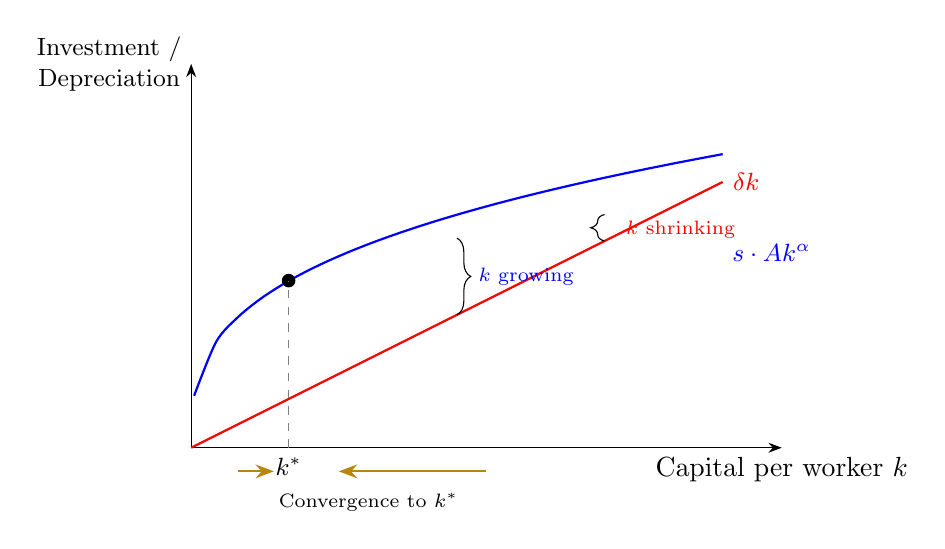
\begin{tikzpicture}[scale=0.75, >=Stealth]
  % Axes
  \draw[->] (0,0) -- (10,0) node[below] {Capital per worker $k$};
  \draw[->] (0,0) -- (0,6.5) node[left, align=center, font=\small]
    {Investment /\\Depreciation};

  % Depreciation: delta*k, linear
  \draw[thick, red] (0,0) -- (9, 4.5)
    node[right, font=\small] {$\delta k$};

  % Investment: s*A*k^alpha, concave
  % s=0.3, A=1, alpha=1/3: s*k^(1/3)
  % at k=0 -> 0; k=1 -> 0.3; k=8 -> 0.6; k=27 -> 0.9; k=64 -> 1.2
  % scale: k axis 0-80 mapped to 0-9; y axis 0-5
  \draw[thick, blue] plot[smooth, domain=0.05:9]
    (\x, {5.0*0.3*(\x/9*80)^(1/3)/1.3});
  \node[right, font=\small, blue] at (9, 3.3) {$s \cdot A k^{\alpha}$};

  % Steady state intersection: k*=14.7 => x = 14.7/80*9 = 1.65
  % s*y* = 0.3 * 14.7^(1/3) = 0.3*2.45 = 0.735 => scaled: 5*0.735/1.3 = 2.83
  % delta*k* = 0.05*14.7 = 0.735 => same
  \filldraw (1.65, 2.83) circle (3pt);
  \draw[dashed, gray] (1.65, 0) -- (1.65, 2.83);
  \node[below, font=\small] at (1.65, 0) {$k^*$};

  % Annotations
  \draw[decorate, decoration={brace, amplitude=5pt, mirror}]
    (4.5, 2.25) -- (4.5, 3.55);
  \node[right, font=\scriptsize, blue] at (4.7, 2.9) {$k$ growing};

  \draw[decorate, decoration={brace, amplitude=5pt}]
    (7.0, 3.5) -- (7.0, 3.95);
  \node[right, font=\scriptsize, red] at (7.2, 3.7) {$k$ shrinking};

  % Arrows showing dynamics
  \draw[->, thick, UoEGold] (0.8, -0.4) -- (1.4, -0.4);
  \draw[->, thick, UoEGold] (5.0, -0.4) -- (2.5, -0.4);
  \node[below, font=\scriptsize] at (3.0, -0.6) {Convergence to $k^*$};
\end{tikzpicture}
\end{center}
\vspace{0.3em}
Below $k^*$: investment $>$ depreciation $\Rightarrow$ capital grows.\\
Above $k^*$: depreciation $>$ investment $\Rightarrow$ capital shrinks.\\
The steady state is \alert{globally stable}.
\end{frame}

\begin{frame}[fragile]{The Solow Diagram in Python}
\begin{lstlisting}
s = 0.3        # saving rate
delta = 0.05   # depreciation rate

k_vals = np.linspace(0, 80, 300)
investment = s * production(k_vals)
depreciation = delta * k_vals

# Steady state: where the curves cross
k_star = (s * A / delta) ** (1 / (1 - alpha))
y_star = production(k_star)
print(f"Steady state: k* = {k_star:.2f}, y* = {y_star:.2f}")
# Output: k* = 14.70, y* = 2.45
\end{lstlisting}
\vspace{0.3em}
At steady state $k^* \approx 14.70$:
\begin{itemize}
  \item Investment = $s \cdot y^* = 0.3 \times 2.45 = 0.735$
  \item Depreciation = $\delta \cdot k^* = 0.05 \times 14.70 = 0.735$
  \item They are \alert{exactly equal} --- capital per worker is constant.
\end{itemize}
\end{frame}

\begin{frame}{Simulating Convergence}
We simulate with Euler integration:
\[
  k_{t+1} = k_t + \Delta t \cdot \bigl(s \cdot A \cdot k_t^{\alpha} - \delta \cdot k_t\bigr)
\]
\begin{center}
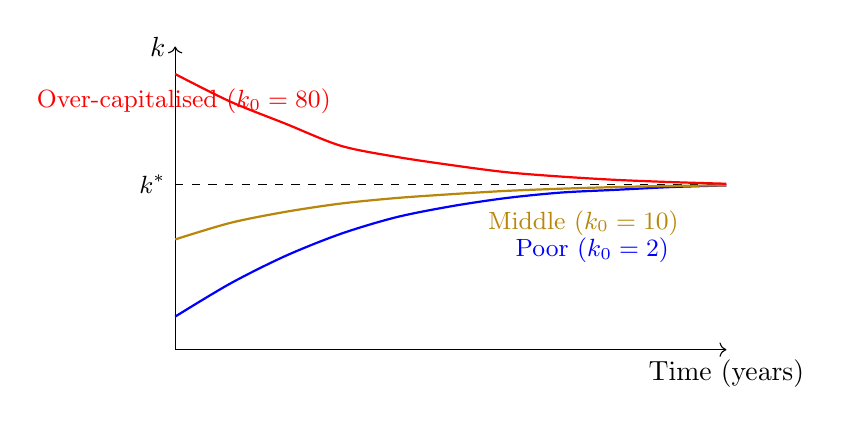
\begin{tikzpicture}[scale=0.7]
  \draw[->] (0,0) -- (10,0) node[below] {Time (years)};
  \draw[->] (0,0) -- (0,5.5) node[left] {$k$};
  % Steady state line
  \draw[dashed, black] (0, 3.0) -- (10, 3.0);
  \node[left, font=\small] at (0, 3.0) {$k^*$};
  % Poor country (k0=2) converging up
  \draw[thick, blue] plot[smooth] coordinates
    {(0,0.6) (1,1.2) (2,1.7) (3,2.1) (4,2.4) (5,2.6) (6,2.75) (7,2.85)
     (8,2.9) (9,2.95) (10,2.98)};
  \node[right, font=\small, blue] at (6, 1.8) {Poor ($k_0 = 2$)};
  % Middle country
  \draw[thick, UoEGold] plot[smooth] coordinates
    {(0,2.0) (1,2.3) (2,2.5) (3,2.65) (4,2.75) (5,2.82) (6,2.88)
     (7,2.92) (8,2.95) (9,2.97) (10,2.98)};
  \node[right, font=\small, UoEGold] at (5.5, 2.3) {Middle ($k_0 = 10$)};
  % Over-capitalised country
  \draw[thick, red] plot[smooth] coordinates
    {(0,5.0) (1,4.5) (2,4.1) (3,3.7) (4,3.5) (5,3.35) (6,3.22)
     (7,3.14) (8,3.08) (9,3.04) (10,3.01)};
  \node[left, font=\small, red] at (3, 4.5) {Over-capitalised ($k_0 = 80$)};
\end{tikzpicture}
\end{center}
Regardless of starting point, all paths converge to $k^*$.
\end{frame}

\begin{frame}[fragile]{Convergence Simulation in Python}
\begin{lstlisting}
def simulate_solow(k0, s, delta, A, alpha, T=200, dt=1.0):
    """Simulate the Solow model from initial capital k0."""
    k = np.zeros(T)
    k[0] = k0
    for t in range(T - 1):
        y = A * k[t]**alpha
        dk = s * y - delta * k[t]
        k[t + 1] = k[t] + dt * dk
    y = A * k**alpha
    c = (1 - s) * y
    return k, y, c

# Simulate from different starting points
for k0 in [2.0, 10.0, 80.0]:
    k, y, c = simulate_solow(k0, s, delta, A, alpha, T=200)
    print(f"k0={k0:5.1f} -> k_final={k[-1]:.2f}")
\end{lstlisting}
\vspace{0.3em}
All three paths converge to $k^* \approx 14.70$:\\
the \alert{fundamental stability property} of the Solow model.
\end{frame}

\begin{frame}{Finding the Steady State Analytically}
At steady state, $dk/dt = 0$:
\[
  s \cdot A \cdot k^{*\alpha} = \delta \cdot k^*
\]
Solving:
\[
  k^{*\,1-\alpha} = \frac{s \cdot A}{\delta}
  \qquad\Longrightarrow\qquad
  \boxed{k^* = \left(\frac{s \cdot A}{\delta}\right)^{\!\frac{1}{1-\alpha}}}
\]
With $s = 0.3$, $A = 1$, $\alpha = 1/3$, $\delta = 0.05$:
\[
  k^* = \left(\frac{0.3}{0.05}\right)^{3/2}
      = 6^{3/2} = 6\sqrt{6} \approx 14.70
\]
\[
  y^* = k^{*1/3} \approx 2.45, \qquad
  c^* = (1-s)\,y^* \approx 1.71
\]
\end{frame}

\begin{frame}[fragile]{Finding the Steady State with \texttt{fsolve}}
\begin{lstlisting}
# Analytical
k_star_analytical = (s * A / delta) ** (1 / (1 - alpha))
print(f"Analytical: k* = {k_star_analytical:.6f}")

# Numerical with fsolve
def solow_equation(k):
    """dk/dt = s*A*k^alpha - delta*k. Zero at steady state."""
    return s * A * k**alpha - delta * k

k_star_numerical = fsolve(solow_equation, x0=10.0)[0]
print(f"Numerical:  k* = {k_star_numerical:.6f}")
print(f"Match: {np.allclose(k_star_analytical, k_star_numerical)}")
\end{lstlisting}
\vspace{0.3em}
\begin{itemize}
  \item \texttt{fsolve} finds where $f(k) = 0$.
  \item Numerical and analytical solutions agree to \textbf{machine precision}.
  \item The numerical approach generalises to models where
        no closed-form solution exists.
\end{itemize}
\end{frame}

\begin{frame}{Comparative Statics: How Parameters Shape the Steady State}
\[
  k^* = \left(\frac{s \cdot A}{\delta}\right)^{\!\frac{1}{1-\alpha}}
\]
\vspace{0.3em}
\begin{columns}[T]
\column{0.32\textwidth}
\begin{block}{Saving rate $s\;\uparrow$}
  Higher $s$ $\Rightarrow$ higher $k^*$ and $y^*$.\\[4pt]
  But consumption $c^*$ first rises, then falls (saving ``too much'').
\end{block}
\column{0.32\textwidth}
\begin{block}{Depreciation $\delta\;\uparrow$}
  Higher $\delta$ $\Rightarrow$ lower $k^*$, $y^*$, $c^*$.\\[4pt]
  Capital wears out faster; the economy is poorer.
\end{block}
\column{0.32\textwidth}
\begin{block}{Technology $A\;\uparrow$}
  Higher $A$ $\Rightarrow$ higher $k^*$, $y^*$, $c^*$.\\[4pt]
  The \alert{only source} of sustained improvement.
\end{block}
\end{columns}
\end{frame}

\begin{frame}[fragile]{Comparative Statics in Python}
\begin{lstlisting}
# Vary saving rate
s_range = np.linspace(0.05, 0.60, 100)
k_star_s = (s_range * A / delta) ** (1 / (1 - alpha))
y_star_s = A * k_star_s**alpha
c_star_s = (1 - s_range) * y_star_s

# Vary depreciation rate
delta_range = np.linspace(0.01, 0.15, 100)
k_star_d = (s * A / delta_range) ** (1 / (1 - alpha))

# Vary technology
A_range = np.linspace(0.5, 3.0, 100)
k_star_A = (s * A_range / delta) ** (1 / (1 - alpha))
\end{lstlisting}
\vspace{0.3em}
Key insight: a higher saving rate raises the \textit{level} of output
but \textbf{not} the long-run \textit{growth rate} (which is zero in
the basic model without technological progress).
\end{frame}

\begin{frame}{The Golden Rule Saving Rate}
Steady-state consumption:
\[
  c^* = y^* - \delta\,k^* = A\,k^{*\alpha} - \delta\,k^*
\]
Maximise with respect to $k^*$:
\[
  \frac{dc^*}{dk^*} = \alpha A\,k^{*\,\alpha - 1} - \delta = 0
\]
\vspace{0.3em}
\textbf{Golden Rule capital:}
\[
  k^*_{GR} = \left(\frac{\alpha A}{\delta}\right)^{\!\frac{1}{1-\alpha}}
\]
\textbf{Golden Rule saving rate:}
\[
  \boxed{s_{GR} = \alpha}
\]
The saving rate that \alert{maximises consumption} equals the
\textbf{capital share of output}.
\end{frame}

\begin{frame}{The Golden Rule Diagram}
\begin{center}
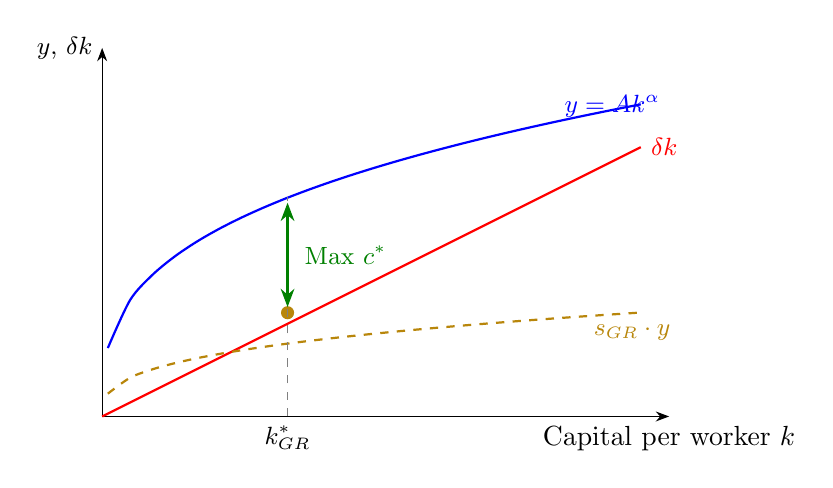
\begin{tikzpicture}[scale=0.72, >=Stealth]
  % Axes
  \draw[->] (0,0) -- (10,0) node[below] {Capital per worker $k$};
  \draw[->] (0,0) -- (0,6.5) node[left, font=\small] {$y$, $\delta k$};

  % Production function y = k^(1/3)
  \draw[thick, blue] plot[smooth, domain=0.1:9.5]
    (\x, {5.5*(\x/9.5*50)^(1/3)/3.68});
  \node[above, font=\small, blue] at (9.0, 5.1) {$y = Ak^{\alpha}$};

  % Depreciation line
  \draw[thick, red] (0,0) -- (9.5, 4.75)
    node[right, font=\small] {$\delta k$};

  % Golden Rule investment: s_GR * y = alpha * y
  \draw[thick, UoEGold, dashed] plot[smooth, domain=0.1:9.5]
    (\x, {5.5*0.333*(\x/9.5*50)^(1/3)/3.68});
  \node[below right, font=\small, UoEGold] at (8.5, 1.8) {$s_{GR} \cdot y$};

  % Golden Rule steady state
  % k*_GR = (alpha*A/delta)^(1/(1-alpha)) = (0.333/0.05)^1.5 = 6.667^1.5 = 17.21
  % x = 17.21/50*9.5 = 3.27
  % delta*k_GR = 0.05*17.21 = 0.861 => scaled = 5.5*0.861/2.585 = 1.83
  % y_GR = 17.21^(1/3) = 2.585 => scaled = 5.5*2.585/3.68 = 3.87
  \filldraw[UoEGold] (3.27, 1.83) circle (3pt);
  \draw[dashed, gray] (3.27, 0) -- (3.27, 3.87);
  \node[below, font=\small] at (3.27, 0) {$k^*_{GR}$};

  % Show max consumption gap
  \draw[<->, thick, green!50!black] (3.27, 1.93) -- (3.27, 3.77);
  \node[right, font=\small, green!50!black] at (3.4, 2.85) {Max $c^*$};
\end{tikzpicture}
\end{center}
\vspace{0.3em}
At the Golden Rule, the gap between $y$ and $\delta k$ is \textbf{largest}
--- consumption per worker is maximised.
\end{frame}

\begin{frame}[fragile]{Golden Rule in Python}
\begin{lstlisting}
s_golden = alpha  # Golden Rule saving rate = capital share
k_golden = (s_golden * A / delta) ** (1 / (1 - alpha))
y_golden = A * k_golden**alpha
c_golden = (1 - s_golden) * y_golden

print(f"Golden Rule: s_GR = {s_golden:.4f}")
print(f"  k*_GR = {k_golden:.4f}")
print(f"  y*_GR = {y_golden:.4f}")
print(f"  c*_GR = {c_golden:.4f}")
\end{lstlisting}
\vspace{0.3em}
\begin{alertblock}{Over-saving}
With $s = 0.30 > s_{GR} = 0.333$?  Actually $s < s_{GR}$ here, so we
under-save slightly.  But if a country saves \textit{more} than $\alpha$,
it is \textbf{dynamically inefficient}: it could consume more
in \textit{every} period by saving less.
\end{alertblock}
\end{frame}

\begin{frame}{Convergence: Poor Countries Grow Faster}
\begin{columns}[T]
\column{0.55\textwidth}
One of the Solow model's most powerful predictions:
\alert{conditional convergence}.
\vspace{0.5em}
\begin{itemize}
  \item Countries far from $k^*$ have \textbf{high} marginal returns
        to capital $\Rightarrow$ grow fast.
  \item Countries near $k^*$ have \textbf{low} marginal returns
        $\Rightarrow$ grow slowly.
  \item This explains the post-war miracles of Germany,
        Japan, and the Asian Tigers.
\end{itemize}
\column{0.4\textwidth}
\begin{center}
\begin{tikzpicture}[scale=0.55, >=Stealth]
  \draw[->] (0,0) -- (8,0) node[below, font=\small] {$k$};
  \draw[->] (0,0) -- (0,6) node[left, font=\small] {Growth rate};
  \draw[thick, UoERed] plot[smooth, domain=0.3:7.5]
    (\x, {5.0/\x});
  \node[right, font=\scriptsize] at (6.5, 1.2) {$\dot{y}/y$};
  \draw[dashed, gray] (0,0) -- (8,0);
  \filldraw[blue] (1.0, 5.0) circle (2pt);
  \node[above, font=\tiny, blue] at (1.0, 5.0) {Poor};
  \filldraw[red] (5.0, 1.0) circle (2pt);
  \node[above, font=\tiny, red] at (5.0, 1.0) {Rich};
\end{tikzpicture}
\end{center}
\end{columns}
\end{frame}

\begin{frame}{Growth Accounting}
Starting from $Y = A K^{\alpha} L^{1-\alpha}$, taking logs and
differentiating:
\[
  \frac{\Delta Y}{Y}
  = \underbrace{\frac{\Delta A}{A}}_{\text{TFP growth}}
  + \alpha \cdot \frac{\Delta K}{K}
  + (1-\alpha) \cdot \frac{\Delta L}{L}
\]
\vspace{0.3em}
The \textbf{Solow residual} (TFP growth) is computed as:
\[
  \frac{\Delta A}{A}
  = \frac{\Delta Y}{Y}
    - \alpha \cdot \frac{\Delta K}{K}
    - (1-\alpha) \cdot \frac{\Delta L}{L}
\]
\vspace{0.3em}
\begin{itemize}
  \item Everything we \textit{can} measure (capital, labour) goes on the right.
  \item Everything we \textit{cannot} measure (technology, institutions,
        management) is captured by the residual.
  \item Solow (1957): the residual accounted for \alert{87.5\%} of US growth.
\end{itemize}
\end{frame}

\begin{frame}{The Population Growth Extension}
With labour force growth at rate $n$, capital is diluted:
\[
  \frac{dk}{dt} = s \cdot A \cdot k^{\alpha} - (\delta + n) \cdot k
\]
The \textbf{break-even investment} line becomes steeper:
\[
  k^* = \left(\frac{s \cdot A}{\delta + n}\right)^{\!\frac{1}{1-\alpha}}
\]
\vspace{0.3em}
\begin{itemize}
  \item Higher population growth $n$ $\Rightarrow$ lower $k^*$ and $y^*$.
  \item Capital must be spread among more workers --- ``capital dilution.''
  \item Countries with rapid population growth tend to have
        \textbf{lower} living standards (per capita), consistent with data.
  \item The Golden Rule saving rate remains $s_{GR} = \alpha$.
\end{itemize}
\end{frame}

% -------------------------------------------------------------
\section{Part III --- Exercises}
% -------------------------------------------------------------

\begin{frame}{Exercise 1: Two-Country Convergence}
Two countries share $A = 1$, $\alpha = 1/3$, $s = 0.25$, $\delta = 0.05$
but start at different capital levels.
\vspace{0.5em}
\begin{enumerate}
  \item Compute the common steady state $k^*$, $y^*$, $c^*$.
  \item Simulate both countries for 150 years from
        $k_0^{\text{poor}} = 2$ (war-ravaged Germany) and
        $k_0^{\text{rich}} = 20$ (the United States).
        Plot $k$ and $y$ over time.
  \item Compute and plot the annual growth rate of $y$ for both.
        When does the poor country's growth rate first fall below 1\%?
  \item Define the \textit{catch-up ratio} $y_{\text{poor}}/y_{\text{rich}}$.
        In approximately what year does the poor country reach 90\%
        of the rich country's output per worker?
\end{enumerate}
\end{frame}

\begin{frame}{Exercise 2: Growth Accounting with Data}
\begin{center}
\begin{tabular}{lccc}
\toprule
Decade & $\Delta Y/Y$ & $\Delta K/K$ & $\Delta L/L$ \\
\midrule
1950s & 7.5\% & 9.0\% & 2.0\% \\
1960s & 6.0\% & 8.0\% & 1.5\% \\
1970s & 4.0\% & 5.5\% & 1.0\% \\
1980s & 3.0\% & 4.0\% & 1.0\% \\
1990s & 2.5\% & 3.0\% & 0.5\% \\
\bottomrule
\end{tabular}
\end{center}
\vspace{0.3em}
Use $\alpha = 1/3$. For each decade:
\begin{enumerate}
  \item Compute the contributions of capital, labour, and TFP growth.
  \item Create a stacked bar chart of the three contributions.
  \item In which decade was TFP growth highest?
  \item This pattern is characteristic of which real-world countries?
\end{enumerate}
\end{frame}

\begin{frame}{Exercise 3: Population Growth Extension}
With population growth at rate $n$:
\[
  \frac{dk}{dt} = s \cdot A \cdot k^{\alpha} - (\delta + n) \cdot k
\]
\vspace{0.3em}
Use $A = 1$, $\alpha = 1/3$, $s = 0.3$, $\delta = 0.05$.
\begin{enumerate}
  \item Derive and compute $k^*$, $y^*$, $c^*$ for $n = 0.02$.
        Verify with \texttt{fsolve}.
  \item Plot the Solow diagram with $(\delta + n)k$ and $\delta k$
        lines on the same graph.
  \item Simulate for $n = 0$, $n = 0.02$, $n = 0.04$.
        What does higher population growth do to steady-state
        living standards?
  \item Derive the Golden Rule when $n > 0$.
        Why does $n$ not affect $s_{GR}$?
\end{enumerate}
\end{frame}

% -------------------------------------------------------------
\section{Key Takeaways}
% -------------------------------------------------------------

\begin{frame}{Quiz: Test Your Understanding}
\begin{enumerate}
  \item Why does capital accumulation alone fail to sustain long-run growth?\\
        \textit{Diminishing returns}: each additional unit of capital
        adds less output.
  \item What does the Solow residual measure?\\
        The fraction of output growth \textbf{not explained} by
        capital and labour growth --- i.e., TFP.
  \item At the steady state, what condition holds?\\
        Investment \textbf{exactly replaces} depreciated capital:
        $s \cdot y^* = \delta \cdot k^*$.
  \item What is the Golden Rule saving rate?\\
        $s_{GR} = \alpha$ --- the capital share of output.
  \item How does the Solow model explain post-war growth miracles?\\
        Countries far below $k^*$ enjoy high returns to capital
        $\Rightarrow$ \alert{rapid convergence}.
\end{enumerate}
\end{frame}

\begin{frame}{What We Learned This Week}
\begin{enumerate}
  \item Robert Solow (1956) showed that \textbf{capital accumulation}
        with diminishing returns leads to a stable \alert{steady state}.
  \item The \textbf{Solow residual} (TFP) accounts for most of observed
        growth --- technology, not saving, is the true engine.
  \item The model predicts \textbf{conditional convergence}: poor countries
        grow faster when they share the same fundamentals.
  \item The \textbf{Golden Rule} $s_{GR} = \alpha$ maximises steady-state
        consumption.
  \item We can \textbf{simulate} the Solow model, find steady states with
        \texttt{fsolve}, and perform \textbf{growth accounting}
        to decompose the sources of growth.
\end{enumerate}
\end{frame}

\begin{frame}{Further Reading}
\begin{itemize}
  \item Solow, R.M. ``A Contribution to the Theory of Economic Growth,''
        \textit{Quarterly Journal of Economics} (1956).
  \item Solow, R.M. ``Technical Change and the Aggregate Production Function,''
        \textit{Review of Economics and Statistics} (1957).
  \item Jones, C.I. \textit{Introduction to Economic Growth}, Chapters~2--3.
  \item Romer, D. \textit{Advanced Macroeconomics}, Chapter~1.
  \item Warsh, D. \textit{Knowledge and the Wealth of Nations}
        (narrative history of growth theory).
\end{itemize}
\vspace{1em}
\begin{center}
\textbf{Next week:} Beyond the Solow Model ---\\
If technology drives growth, where does technology come from?\\
Endogenous growth theory and the economics of innovation.
\end{center}
\end{frame}

\end{document}
